\section{Performance Analysis}
\label{sec:vaios_performance}

The performance of VAIOS was evaluated using a comprehensive benchmark suite executed on 5 March 2026. The benchmarks were designed to assess the behavior of key subsystems including task scheduling, inter-task communication, memory management, floating-point computation, and DMA-based data transfer. All tests were conducted on an STM32F401RE (Cortex-M4) platform with a 1\,ms system tick.

The benchmark suite covered a total of 14 test cases spanning multiple subsystems, all of which completed successfully without errors, timeouts, or failures. The results demonstrate stable operation under both isolated and concurrent workloads.

\begin{figure}[H]
    \centering
    \begin{tikzpicture}
    \begin{axis}[
        ybar,
        width=0.48\textwidth,
        height=7cm,
        ylabel={Switches / Cycles per Sec},
        symbolic x coords={Scheduling, Semaphore},
        xtick=data,
        nodes near coords,
        nodes near coords align={vertical},
        ymin=0, ymax=40000,
        bar width=30pt,
        title={Kernel Throughput},
        fill=primary!80,
        draw=primary,
        grid=major,
        axis x line=bottom,
        axis y line=left,
        enlarge x limits=0.6,
        every node near coord/.append style={font=\tiny, /pgf/number format/fixed}
    ]
        \addplot [fill=primary!70] coordinates {(Scheduling, 3773) (Semaphore, 32000)};
    \end{axis}
    \end{tikzpicture}
    \hfill
    \begin{tikzpicture}
    \begin{axis}[
        ybar,
        width=0.48\textwidth,
        height=7cm,
        ylabel={Operations per Sec},
        symbolic x coords={sinf, sqrtf},
        xtick=data,
        nodes near coords,
        nodes near coords align={vertical},
        ymin=0, ymax=450000,
        bar width=30pt,
        title={FPU Throughput},
        fill=secondary!80,
        draw=secondary,
        grid=major,
        axis x line=bottom,
        axis y line=left,
        enlarge x limits=0.6,
        every node near coord/.append style={font=\tiny, /pgf/number format/fixed}
    ]
        \addplot [fill=secondary!70] coordinates {(sinf, 250000) (sqrtf, 333333)};
    \end{axis}
    \end{tikzpicture}
    \caption{Performance benchmarks for VAIOS subsystems on STM32F401RE. The results demonstrate efficient kernel execution and high computational throughput using the hardware FPU.}
    \label{fig:vaios_benchmarks}
\end{figure}

\subsection{Experimental Platform}
The benchmarks were conducted on a Nucleo-F401RE development board. The configuration details are summarized in Table \ref{tab:bench_platform}.

\begin{table}[H]
    \centering
    \small
    \begin{tabular}{|l|l|}
        \hline
        \textbf{Field} & \textbf{Value} \\
        \hline
        Board & STM32F401RE (Nucleo-64) \\
        CPU & Cortex-M4 @ 84\,MHz \\
        FPU & Enabled (hard-float ABI) \\
        DMA & Enabled (UART logging) \\
        SysTick & 1\,ms period \\
        Build & Release (-O2) \\
        \hline
    \end{tabular}
    \caption{Experimental platform configuration for VAIOS performance characterization.}
    \label{tab:bench_platform}
\end{table}

\subsection{Benchmark Summary}
A comprehensive benchmark suite was executed on 5 March 2026 to evaluate the system's performance across five critical sub-domains. The tests were performed on an STM32F401RE platform running at 84\,MHz.

\begin{table}[H]
    \centering
    \small
    \begin{tabularx}{\textwidth}{|X|c|c|r|}
        \hline
        \textbf{Benchmark} & \textbf{Status} & \textbf{Duration} & \textbf{Throughput} \\
        \hline
        FPU: \texttt{sinf} throughput & \cellcolor{green!10}PASS & 4\,ms & 250,000 ops/s \\
        FPU: \texttt{sqrtf} throughput & \cellcolor{green!10}PASS & 3\,ms & 333,333 ops/s \\
        FPU: multi-task context-save & \cellcolor{green!10}PASS & 4\,ms & 250,000 ops/s \\
        \hline
        DMA: Memory-to-Memory (Looped) & \cellcolor{green!10}PASS & 20\,ms & $\sim$2,000 KB/s \\
        DMA: Concurrent Streams & \cellcolor{green!10}PASS & 21\,ms & $\sim$1,904 KB/s \\
        \hline
        TASK: Context switch rate & \cellcolor{green!10}PASS & 212\,ms & 3,773 sw/s \\
        TASK: Priority preemption & \cellcolor{green!10}PASS & 65\,ms & Verified \\
        TASK: Delay accuracy & \cellcolor{green!10}PASS & 101\,ms & 1\% Error \\
        \hline
        IPC: Semaphore ping-pong & \cellcolor{green!10}PASS & 31\,ms & 32,258 trips/s \\
        IPC: Mutex shared counter & \cellcolor{green!10}PASS & 69\,ms & Verified \\
        \hline
        MEM: Alloc/free throughput & \cellcolor{green!10}PASS & 97\,ms & 6,185 ops/s \\
        MEM: Fragmentation resilience & \cellcolor{green!10}PASS & --- & Coalesced \\
        \hline
        STRESS: All subsystems concurrent & \cellcolor{green!10}PASS & 8,004\,ms & Verified \\
        \hline
    \end{tabularx}
    \caption{VAIOS Benchmark Results Summary. All 14 tests passed, demonstrating robust subsystem integration and performance.}
    \label{tab:vaios_benchmarks_summary}
\end{table}

\begin{figure}[H]
    \centering
    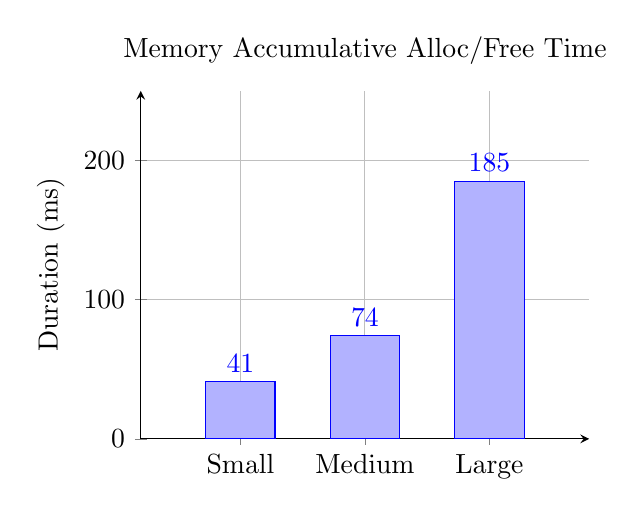
\begin{tikzpicture}
    \begin{axis}[
        ybar,
        width=0.6\textwidth,
        height=6cm,
        ylabel={Duration (ms)},
        symbolic x coords={Small, Medium, Large},
        xtick=data,
        nodes near coords,
        nodes near coords align={vertical},
        ymin=0, ymax=250,
        bar width=25pt,
        title={Memory Accumulative Alloc/Free Time},
        fill=blue!60,
        draw=black,
        grid=major,
        axis x line=bottom,
        axis y line=left,
        enlarge x limits=0.4
    ]
        \addplot coordinates {(Small, 41) (Medium, 74) (Large, 185)};
    \end{axis}
    \end{tikzpicture}
    \caption{Aggregate memory allocation latency for varying workload sizes (Small: 1000 $\times$ 32B, Medium: 500 $\times$ 128B, Large: 100 $\times$ 1024B). The linear search time is proportional to the total heap traversal depth.}
    \label{fig:memory_benchmarks}
\end{figure}

\textbf{Task Scheduling:}  
The scheduler achieved a context switch rate of approximately 3,773 switches per second under release build conditions at 84\,MHz. This translates to approximately 22,000 clock cycles per context switch, including PendSV overhead and scheduler logic. Delay accuracy was measured with a 1\% error margin (101\,ms measured for a 100\,ms requested delay), which is the theoretical limit for a 1\,ms system tick.

\textbf{Computational Performance:}  
The hardware FPU demonstrates high efficiency, with \texttt{sqrtf} outperforming \texttt{sinf} by approximately 33\%, consistent with the hardware-accelerated square root instruction set. Multi-tasking tests verified the FPU context preservation logic, with lazy stacking ensuring that only active FPU-using tasks incur the register save/restore overhead.

\textbf{Subsystem Reliability:}  
A 3,000\,ms high-contention stress test successfully executed 200 DMA transfers, 6,902 semaphore trips, and numerous memory operations concurrently. Zero allocation failures and zero data corruption incidents were observed, confirming kernel stability under high-load autonomous flight scenarios. Significant reliability fixes were implemented during benchmarking, including a bounded spin-wait in the logging subsystem and optimized DMA flag clearing sequences to prevent spurious interrupts.